%Fiquemos com Deus e Nossa Senhora!
\documentclass[journal]{IEEEtran}

\usepackage{amsmath,algorithmic,url,color}

% correct bad hyphenation here
\hyphenation{op-tical net-works semi-conduc-tor}


\begin{document}

\title{FEMa: A Finite Element Machine for Fast Learning}

\author{Danillo~Roberto~Pereira,        
		Jo\~ao~Paulo~Papa,~\IEEEmembership{Member,~IEEE,}
        and~Hojjat~Adeli,~\IEEEmembership{Member,~IEEE}% <-this % stops a space
\thanks{D. Pareira and J. Papa are with the Department
of Computing, S\~ao Paulo State University, Bauru, SP, 17033-360
 Brazil e-mail: dpereira@ic.unicamp.br, papa@fc.unesp.br.}% <-this % stops a space
\thanks{H. Adeli is with the Department of Civil, Environmental and Geodetic Engineering, The Ohio State University, Columbus, OH 43210 USA e-mail: adeli.1@osu.edu}% <-this % stops a space
\thanks{Manuscript received April 19, 2005; revised August 26, 2015.}}

\markboth{Journal of \LaTeX\ Class Files,~Vol.~14, No.~8, August~2015}%
{Shell \MakeLowercase{\textit{et al.}}: Bare Demo of IEEEtran.cls for IEEE Journals}

\maketitle

\begin{abstract}
\end{abstract}

\begin{IEEEkeywords}
Finite Element Method, Classification, Regression.
\end{IEEEkeywords}

\IEEEpeerreviewmaketitle

\section{Introduction}
\label{s.introduction}

\IEEEPARstart{T}{he} ``Big Data"\ era has flooded researchers and the whole community with tons of data daily. Multimedia-based applications are in charge of generating an unsurmountable amount of data, which end up at the screens of mobile phones and tablets. Home-made videos are usually referred as the bottleneck of any network traffic analyzer, since they are uploaded to cloud-driven servers as soon as they are generated or forwarded by someone else via the so-called social networks.

The huge amount of data requires to be processed and mined efficiently. Former versions of well-known machine learning techniques such as Support Vector Machines (SVMs)~\cite{CortesML:95}, Artificial Neural Networks (ANNs)~\cite{HungNeuro:93,AdeliMLN:94}, Polynomial Neural Networks~\cite{LinTSMCS:15a}, Recurrent Networks~\cite{LinTSMCS:15b,LiuTSMCS:16}, and Adaptive Conjugate Gradient Neural Networks~\cite{AdeliAMC:94,AdeliJSA:93} are now being implemented in General-Purpose Computing on Graphics Processing Units (GPGPU) to cope with streams of data that need to be analyzed daily.

Active learning is another research area that needs fast techniques for learning and classification. One very usual example concerns interactive and semi-supervised learning tools for image classification and annotation. Suppose a physician wants to classify a Magnetic Resonance image of the brain, which may contain hundreds of thousands of pixels. The user shall mark a few positive and negative samples (pixels) that will be used to train the classifier, which then classifies the remaining image. Further, the user shall refine the results by marking some misclassified regions for training once more. Notice the whole process should take a few seconds/iterations. In this context, the user feedback is crucial to obtain a concise/reliable labeled image.

Considering the aforementioned situation, some techniques may not be appropriate to be employed, since they can hardly handle the problem of updating the model learned previously when new training samples come to the problem. Support Vector Machines are known to be costly, since they require a fine-tuning parameter step, which turns out to be the bottleneck for efficient implementations~\cite{ChouCACIE:15}. Although different variations and GPU-based implementations are published monthly, it is not straightforward to use them, which makes them far from being user-friendly. Additionally, SVM training step is quadratic with respect to the number of training examples.

Deep learning techniques have have received a lot of attention in recent years~\cite{LeCunNature:15,RafieiCEM:16}, since they can learn features from images/signals without label information. Although such approaches have obtained outstanding results in a number of applications, they usually overfit under small training sets. Also, some architectures require hundreds of parameters for fine-tuning resulting in very costly training.

Graph-based pattern recognition techniques took their place in the scientific community as well. Papa et al.~\cite{PapaISVC:08,PapaIJIST:09,PapaPR:12,PapaPRL:17} proposed the Optimum-Path Forest (OPF), a framework for the design of classifiers. OPF has obtained promising results in a number of applications, being much faster than SVM for training, since its original version is parameterless~\cite{PapaIJIST:09,PapaPR:12} and does not require fine-tuning parameters. However, OPF-based classifiers are usually affected by high-dimensional spaces, a shortcoming for techniques that make use of distances for classification purposes.

Artificial Neural Networks have been reinvented in the last decades. From the original Backpropagation learning algorithm~\cite{RumelhartNature:86} to faster approaches such as the Levenberg-Marquardt~\cite{HaganIEEETNN:94}, the reader can refer to a number of variants that somehow try to deal with the problem of avoiding getting trapped from local optima during training, as well as to make their convergence step faster~\cite{LiuIEEETSMC:11}. Polynomial neural networks~\cite{Lin:15}, hybrid networks~\cite{Martinel:15}, and probabilistic ones~\cite{Specht:90,AhmadlouICAE:10} have been used in a number of different applications in the literature.



In early 90's, Specht~\cite{Specht:90} proposed the Probabilistic Neural Networks (PNNs), which basically replaces the sigmoid activation function by an exponential one. Since PNNs do not require using Backpropagation, they are usually much faster than traditional ANNs~\cite{AdeliNN:09,SankariJNM:11}. PNNs are composed of four layers: input, pattern, summation and output. The first layer is responsible for feeding the network with features extracted from samples, and the pattern layer aims at encoding all training data patterns, i.e. the number of pattern units (Gaussian probability distribution functions) is the very same number of training samples. The summation layer contains one unit for each class, and the output layer uses a Bayesian rule to compute the probability in assigning a certain class to a given input data. Since standard PNNs use an exponential activation function, one needs to set the variance (spread) of the Gaussian function, which can considerably influence the effectiveness of the network. 

Some years later, Ahmadlou and Adeli~\cite{AhmadlouICAE:10} proposed the Enhanced Probabilistic Networks (EPNNs), a clever way to penalize outliers when computing the influence of the Gaussian distribution over the training samples. Actually, the authors proposed to compute a variance for each training sample based on a neighborhood, and depending on the class labels of its neighbours, the Gaussian function centered at an outlier pattern can barely influence other points. Papers that make use of EPNNs have appeared in the literature~\cite{Sankari:11,Hirschauer:15}, since EPNNs are fast and very suitable for large-scale datasets.

Moving from machine learning to numerical analysis, one of the most widely used approaches for finding approximate solutions to boundary-value problems in partial differential equations is the Finite Element Method (FEM)~\cite{Zienkiewicz:67,YuJSE:93}. Roughly speaking, FEM divides the original problem into smaller pieces called finite elements, and the simple equations that describe each element are assembled in a complex one that should describe the whole problem. Therefore, given a set of points, FEM can interpolate them using basis functions in order to build a manifold that contains all these points. In this paper, we borrow some ideas related to FEM to propose FEMa - Finite Element Machine, a new framework for the design of pattern classifiers based on finite element analysis. Depending on the basis function used, FEMa can be parameterless. It features a quadratic complexity for both training and classification phases, which turns out to be its main advantage when dealing with massive amount of data. In short, FEMa learns a probabilistic manifold built over the training samples, which are the center of a finite element basis. Therefore, the problem of learning a manifold using one finite element basis is broken into a surface composed of several bases, centered at each training sample. In this paper, we show that FEMa can obtain very competitive results when compared against some state-of-the-art supervised pattern recognition techniques.

The remainder of this paper is organized as follows. Sections~\ref{s.fem} and~\ref{s.fema} introduce the theoretical background related to FEM and FEMa, respectively. Section~\ref{s.methodology} presents the methodology and experiments used to evaluate FEMa in the context of big data environments, and Section~\ref{s.conclusions} states conclusions and future works.
\section{Finite Element Machine}
\label{s.fema}

In this section, we present the Finite Element Machine classifier, as well as how it can cope with the problem of supervised pattern classification efficiently. \textcolor{blue}{In this point is import highlight that FEMa is not a generalization of the variation o k-NN (k-Nearest Neighbour) or w-NN (Weighted Nearest Neighbour)~\cite{Samworth:12} even w-NN can being seen as an special case of the FEMa. So it is very important emphasize that FEMa has all fundamental background based on Finite Element Method . The FEMa allows work with a huge number of different basis, as: Radial Basis Function, Normalized Radial Basis Function and many others. All the background developed in this work provides a elegant solutions for basis which are neither interpolating and not partition-unit basis.  FEMa opens a wide range of new studies of finite element bases applied in machine learning.}

\subsection{Background Theory}
\label{ss.background}

Let ${\cal Z}={\cal Z}_1\cup{\cal Z}_2$ be a dataset partitioned into a training (${\cal Z}_1$) and a test (${\cal Z}_2$) set. In this case, the pair $(\textbf{x}_i,y_i)\in{\cal Z}$ denotes the feature vector $\textbf{x}_i\in\Re^m$ extracted from sample $i$, and $y_i$ stands for its label. Notice we adopted the very same formulation used in the previous section, i.e. a point in FEM formulation stands for a sample in FEMa.

Roughly speaking, FEMa learns a set of probability functions ${\cal P}(\textbf{x})=\{P_1(\textbf{x}),P_2(\textbf{x}),\ldots,P_c(\textbf{x})\}$, where $c$ stands for the number of classes, and $P_i(\textbf{x})$ represents the probability of a given sample $\textbf{x}$ to be assigned to class $i$. In other words, FEMa aims at learning a probabilistic manifold from the training set.

\subsection{Probabilistic Manifold Learning}
\label{ss.manifold}

Depending on the basis function used to interpolate points, FEMa does not require a training step, which turns out to be quite interesting when dealing with big data. Precisely, this assumption is true concerning bases that are natively interpolating, such as Shepard basis. On the other hand, with respect to non-interpolating basis, e.g. radial functions, one needs to compute $\textbf{Z}^{-1}$ in Equation~\ref{e.interpolating_basis}. Also, if the basis function does not hold the partition of unity property, one shall compute Equation~\ref{e.normalization} either. Therefore, although FEMa can be used with any basis function, we shed light over that bases holding both the interpolating and partition of unity properties are much more appealing when dealing with massive amount of data. As such, we can consider the calculation of $\textbf{Z}^{-1}$ and Equation~\ref{e.normalization} as the training steps when using non-interpolating and non-partition of units bases.

Assuming we are using an interpolating and partition of unity basis (e.g Shepard), we can move to the classification step. Given a sample $\textbf{x}\in{\cal Z}_2$, we need to compute its probability of belonging to each class $i$, $i=1,2,\ldots,c$, as follows:

\begin{equation}
	P_i(\textbf{x})=\sum_{j=1}^{\left|{\cal Z}_1\right|}\rho_i^j\phi_j(\textbf{x}),
\end{equation}
where $\rho_i^j\in[0,1]$ stands for the probability of training sample $j$ belonging to class $i$. An interesting property concerning FEMa relates to the possibility in assigning a probability to each training sample, which means we have an uncertainty associated to those samples, thus having an important role when dealing with data overfitting. This capability is extremely important in medical-driven applications, where physicians usually have different opinions with respect to the very same data (e.g. cancer detection in images).

The probability $\rho_i^j\in[0,1]$ can be computed using the following formulation:

\begin{equation}
\rho_i^j =  \left\{
			  \begin{array}{ll}
			      1 & \hbox{if $y_{j} = i$}\\
			      0 & \hbox{otherwise.}\\
			  \end{array}
		    \right.
\end{equation}
Since we have labeled datasets (i.e. we are assuming the labeling process is errorless), we can use $\rho_i^j\in\{0,1\}$. Therefore, we generate the set of probabilities ${\cal P}(\textbf{x})$ for each sample $\textbf{x}\in{\cal Z}_2$. 

In short, FEMa classifies a given sample $\textbf{x}\in{\cal Z}_2$ as belonging to the class $\hat{y}$ that satisfies the above equation:

\begin{equation}
	\hat{y} = \arg\max_{i}P_i(\textbf{x}).
\end{equation}
Also, FEMa allows us to infer the certainty $C(\textbf{x})$ as follows:

\begin{equation}
\label{eq.certainty}
	C(\textbf{x})=\frac{P_{\hat{y}}(\textbf{x})}{\sum_{j=1}^cP_j(\textbf{x})}.
\end{equation}
Therefore, FEMa can produce both hard and soft (probability) outputs without any modification. Figure~\ref{fig.ProbFunc} illustrates the process of learning the probability functions of each class in a one-dimensional and two-class problem. For the sake of explanation, the $x$-axis stands for a test set with samples within the interval $[-3,3]$, and the $y$-axis denotes their probability values with respect to the class $1$ (Figure~\ref{fig.ProbFunc}a) and class $2$ (Figure~\ref{fig.ProbFunc}b). Also, the red dots stand for the training samples, i.e. the centers of the basis functions.

Let us consider a test sample with value $-2$ in Figure~\ref{fig.ProbFunc}c. As one can observe, such sample has been used as a center for the basis function in Figure~\ref{fig.ProbFunc}a already (it is a training sample). In this case, the classification process will assign class $1$ to this sample, since $P_1(-2)\approx 1$, and $P_2(-2)\approx 0$. Now, consider a sample with value $2$ that does not belong to the training set, i.e. it is not a basis center. In this case, $P_1(2)\approx 0.15$ and $P_2(2)\approx 0.85$, which leads FEMa to assign class $2$ to that sample.

\begin{figure}[!htb]
\centering
\begin{tabular}{cc}
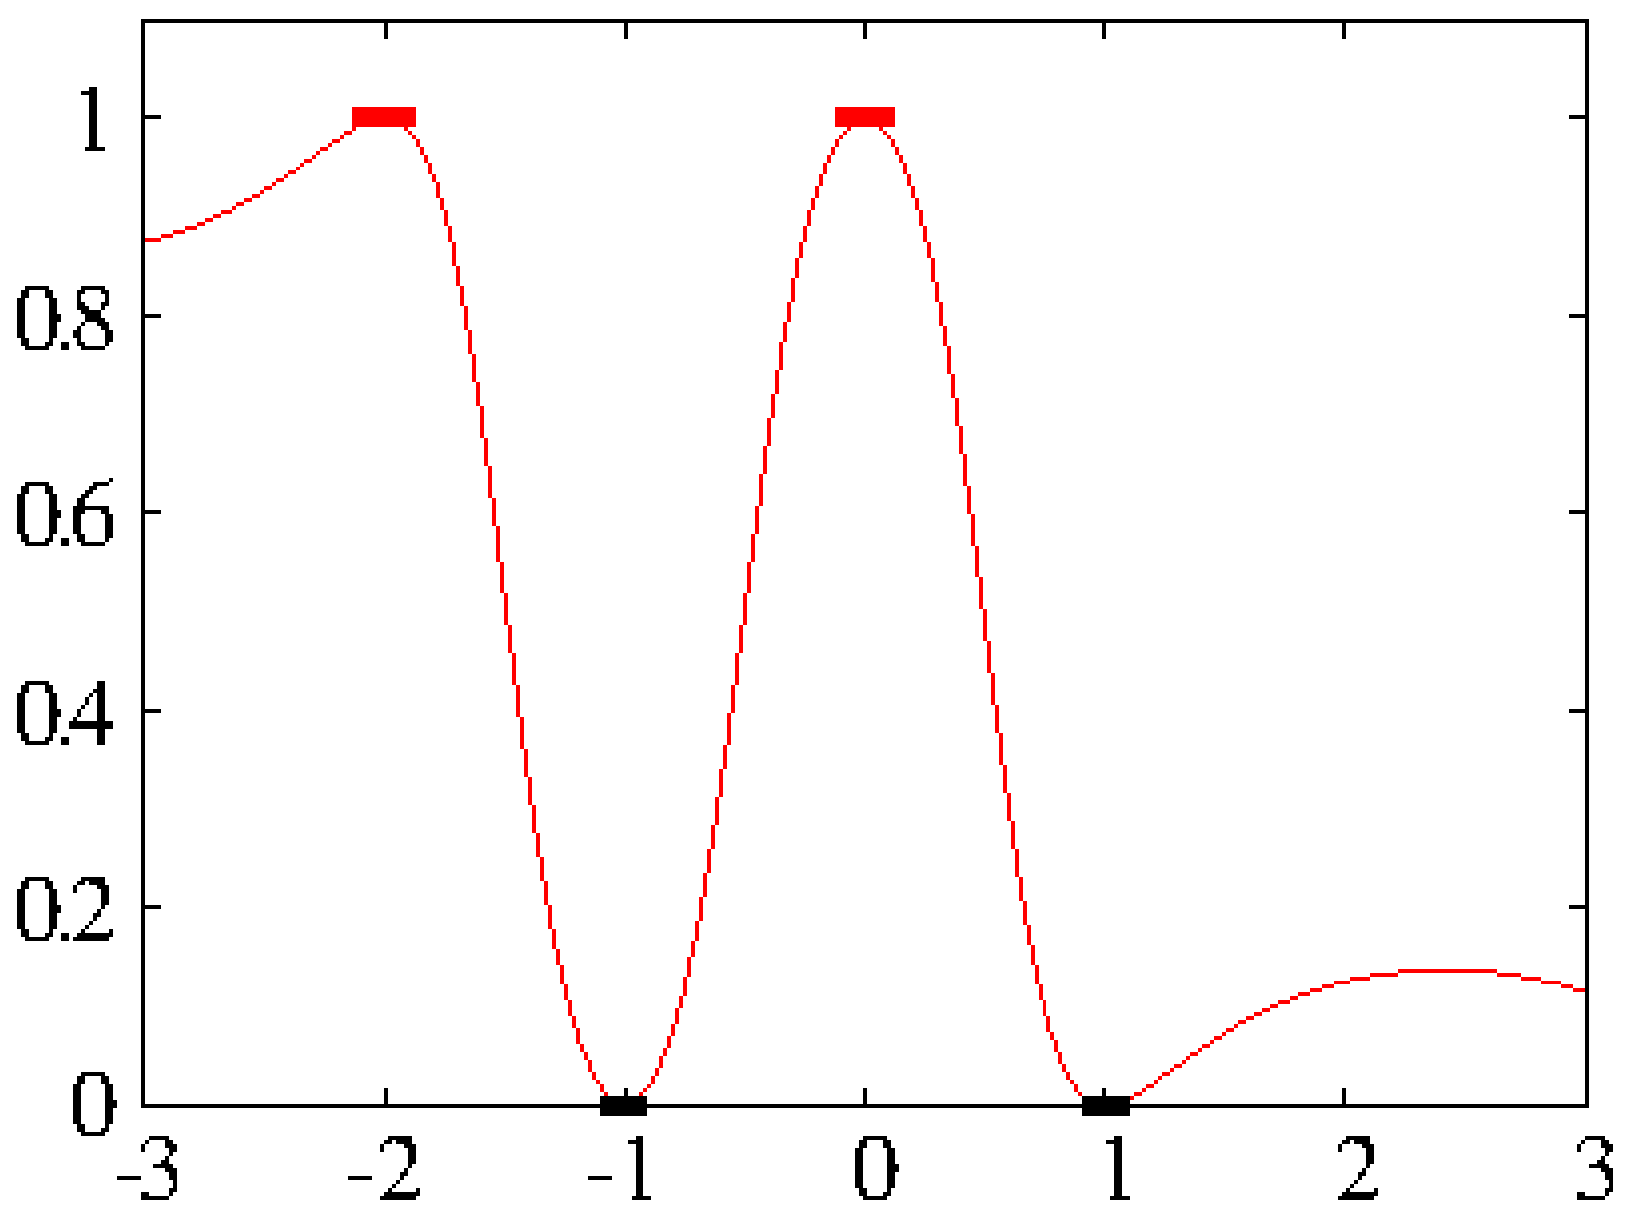
\includegraphics[scale=0.153]{./ShepardClass1.eps} &
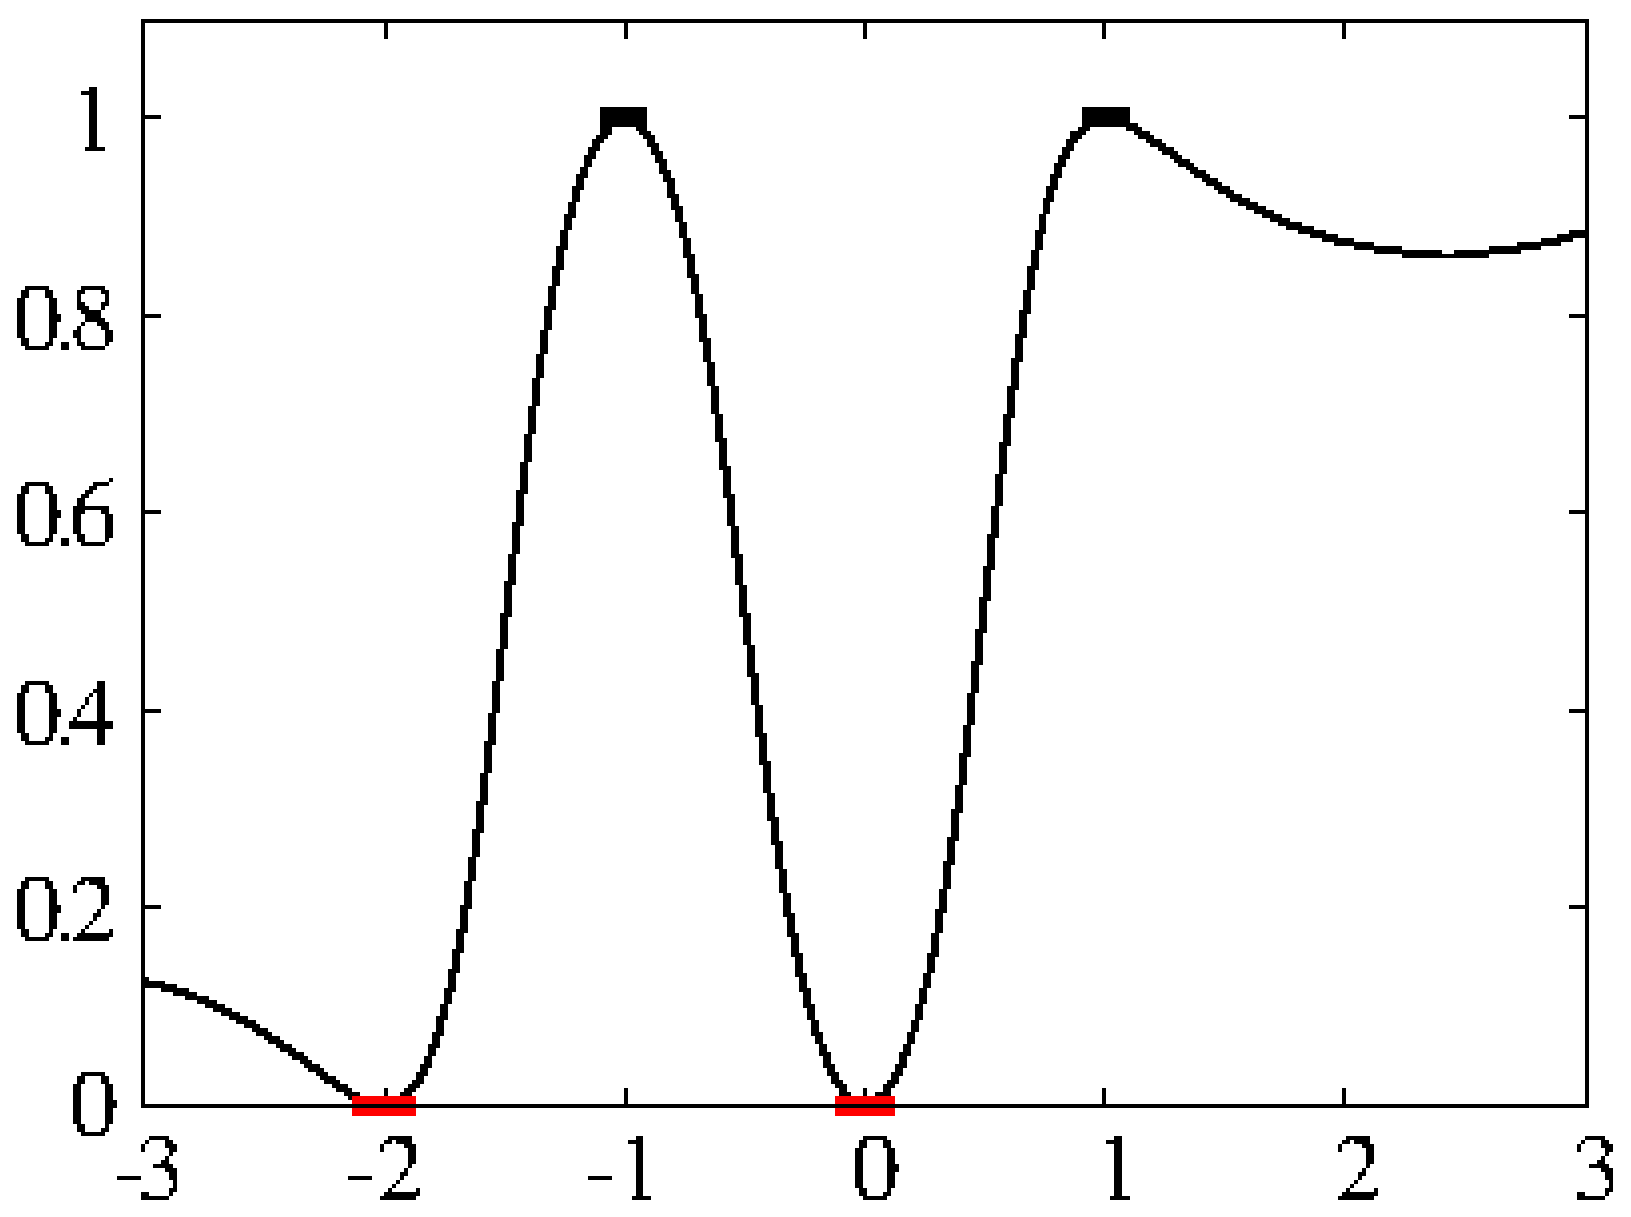
\includegraphics[scale=0.153]{./ShepardClass2.eps} \\
(a) & (b)\\
\end{tabular}
\begin{tabular}{c}
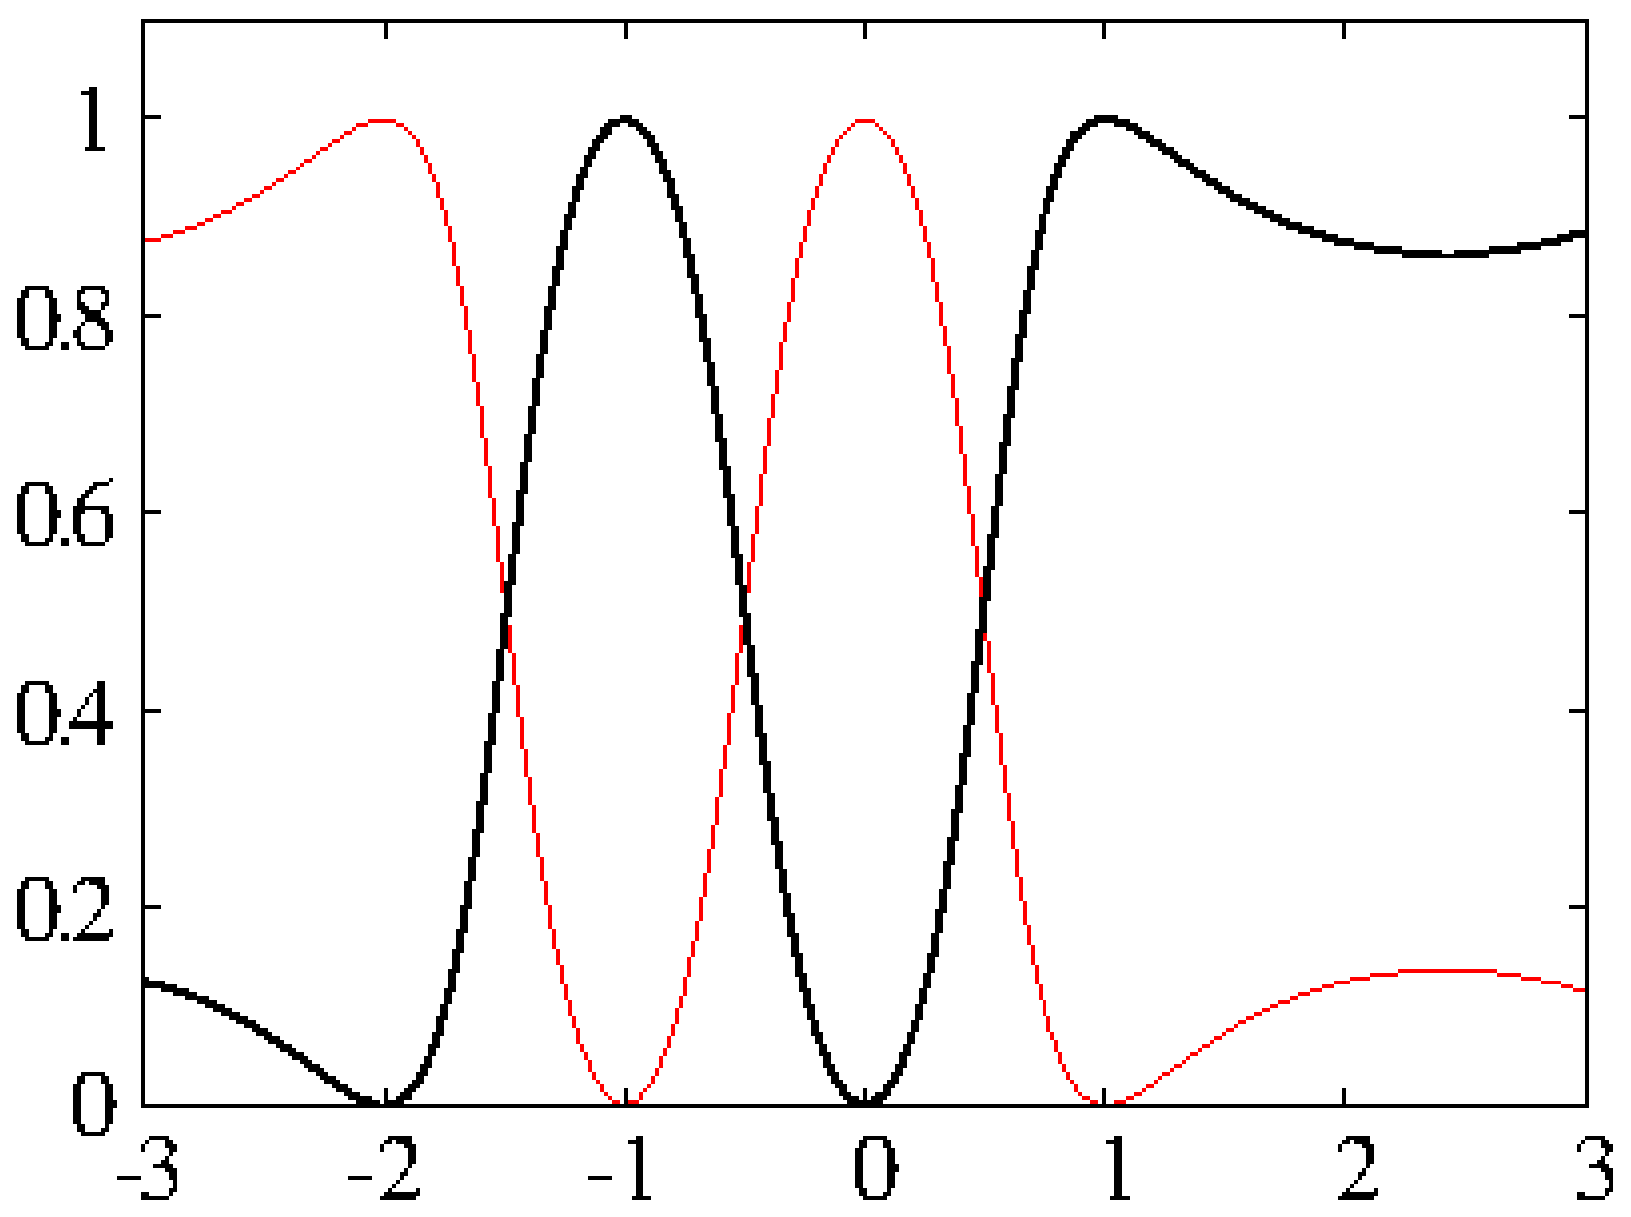
\includegraphics[scale=0.153]{./ShepardProbClass.eps} \\
(c)
\end{tabular}
\caption{The Shepard approximation of the probability function of a two-class problem using $k=3$ considering a given sample $\textbf{x}$: (a) $P_1(\textbf{x})$ and (b) $P_2(\textbf{x})$. The red dots and the red curve denote the samples and the probability function of class $1$, respectively, and the black dots and the black curve stand for the samples and the probability function of class $2$, respectively. In (c), we have the two probability functions together. Notice each real number in $[-3,3]$ (i.e. $x$-axis) is classified according to the class that has the higher probability value (i.e. $y$-axis).}
\label{fig.ProbFunc}
\end{figure}

\subsection{Toy Example}
\label{ss.toy}

In this section, we present the FEMa working mechanism on a bidimensional classification problem. Figure~\ref{2Dpoints}a shows a training set with samples distributed over three classes (red, green and blue). The task is to verify the influence region of each training sample in the image domain, i.e. to classify the remaining points (white ones) in the image frame displayed in Figure~\ref{2Dpoints}a. In this case, the feature of each sample (point) is just its $(x,y)$-position.

\begin{figure}[!htb]
\centering
\begin{tabular}{cc}
\hspace{0.31cm}\moldura{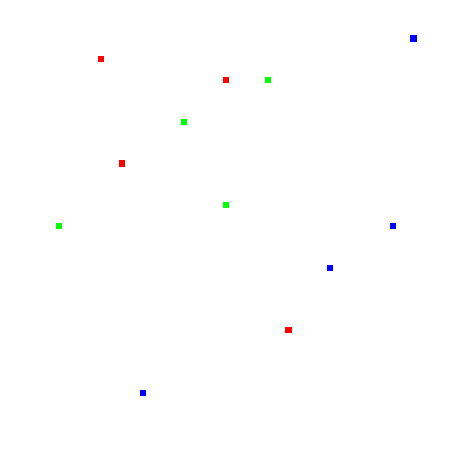
\includegraphics[width=3.39cm]{./points.eps}} &
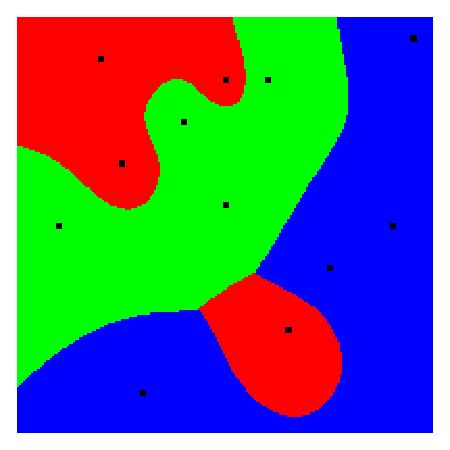
\includegraphics[width=3.39cm]{./out_p1.eps} \\
(a) & (b)\\
\end{tabular}\newline
\begin{tabular}{cc}
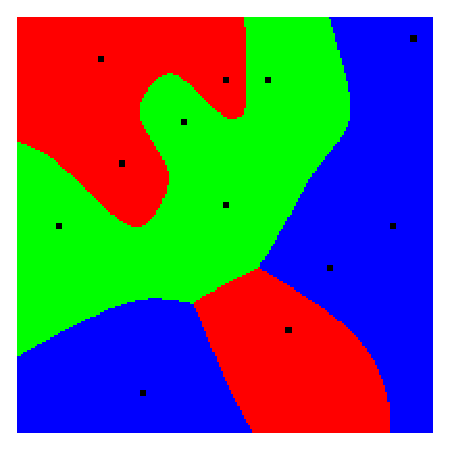
\includegraphics[width=3.39cm]{./out_p3.eps} &
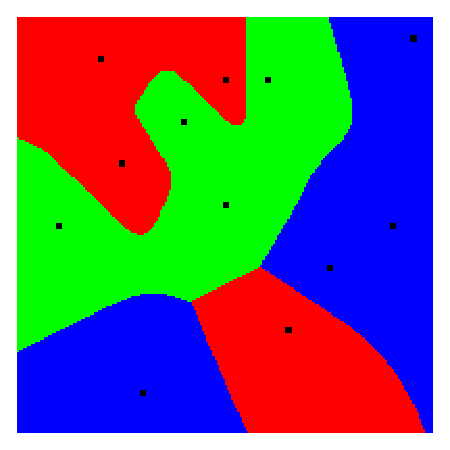
\includegraphics[width=3.39cm]{./out_p5.eps} \\
(c) & (d)\\
\end{tabular}
\caption{FEMa working mechanism: (a) training set with samples distributed in three classes, and the image classified by FEMa using (b) $k=1$, (c) $k=3$ and (d) $k=5$.}
\label{2Dpoints}
\end{figure}

Figures~\ref{2Dpoints}b,~\ref{2Dpoints}c and~\ref{2Dpoints}d depict the image frame classified by FEMa using the Shepard basis with $k=1$, $k=3$ and $k=5$, respectively. Since we are using the $(x,y)$ coordinates to describe each sample, the labeled image refers to the influence region of each training sample, which ends up generating the boundaries of each class. Notice that FEMa can obtain quite good and smooth decision boundaries for different values of $k$ (Equation~\ref{eq.w}). As matter of fact, the larger the value of $k$, the less points will influence the interpolating process of the probability function. For the sake of clarification purposes, when $k\to\infty$, FEMa tends to behave similarly to the well-known nearest neighbor classifier.

Figure~\ref{fig.2Dcertain}a displays the degree of certainty (Equation~\ref{eq.certainty}) computed by FEMa with $k=3$ for each test sample with respect to Figure~\ref{2Dpoints}a. The brighter the pixel, the greater its degree of certainty to be assigned to some class. Notice the darker pixels fall in the boundary among classes (Figure~\ref{2Dpoints}c). Figure~\ref{fig.2Dcertain}b represents each test sample by its label color weighted by its degree of certainty.

\begin{figure}[!htb]
\centering
\begin{tabular}{cc}
 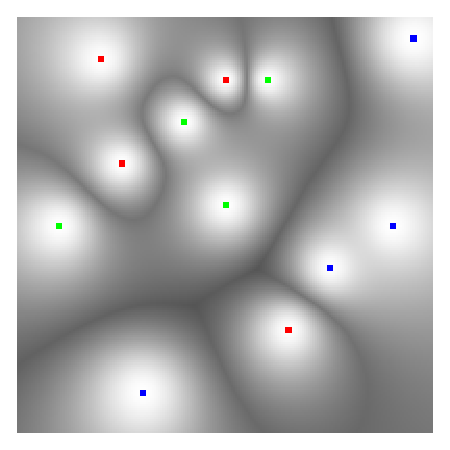
\includegraphics[scale=0.5]{./certain_p.eps} &
 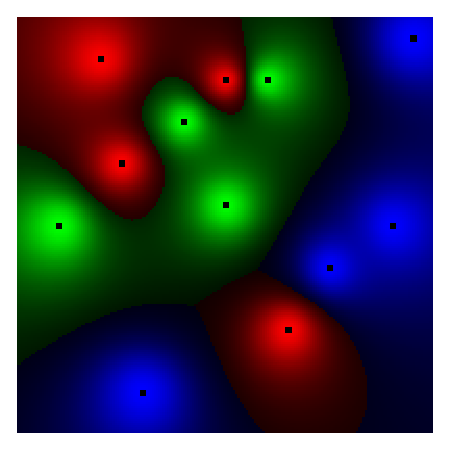
\includegraphics[scale=0.5]{./out_w_p.eps} \\
 (a) & (b)
 \end{tabular} 
 \caption{Probability map (degree of certainty) computed by FEMa in (a), and the test samples with their class label weighted by their respective degree of certainty.}
   \label{fig.2Dcertain}
\end{figure}

\subsection{Complexity Analysis}
\label{ss.complexity}

As aforementioned, depending on the basis function used to build the probabilistic manifold (i.e. interpolating and partition of unity properties), FEMa does not require an explicit training step, since we just need to place the training points, thus taking $\theta(1)$. However, if one uses a non-interpolating basis function, we need to compute the inverse matrix $\textbf{Z}^{-1}$ in Equation~\ref{e.interpolating_basis}, which requires $\theta(\left|{\cal Z}_1\right|^{2.37})$ using the Coppersmith-Winograd algorithm~\cite{Coppersmith:90}.

In regard to the classification phase, for each test sample $\textbf{x}$, we need to compute Equation~\ref{eq.shepard_basis}, which requires $\theta({\left|{\cal Z}_1\right|})$. However, the denominator of such equation considers all training samples, thus becoming a constant, and we need to compute it only once. Since the test set contains $\left|{\cal Z}_2\right|$ samples, the overall classification phase takes $\theta(\left|{\cal Z}_1\right|+\left|{\cal Z}_1\right|\left|{\cal Z}_2\right|)\in\theta(\left|{\cal Z}_1\right|.\left|{\cal Z}_2\right|)$. Therefore, by using an interpolating basis function, the whole FEMa learning and classification processes require a quadratic complexity with respect to the training/testing set size (i.e. when $\left|{\cal Z}_1\right|=\left|{\cal Z}_2\right|$).

However, when we have unbalanced datasets, samples from the majority classes will have a stronger influence when computing the probability functions. Suppose a two-class classification problem, i.e. we have samples from the positive and negative samples. Also, suppose samples from the negative class comprise only $1\%$ of the number of positive samples. When we are computing the probability function of test sample, the positive samples will play a major role during this computation process. In order to overcome this problem, we can use only the $T$ nearest training samples from each class, where $T\in O(\alpha)$ and $\alpha$ stands for the number of elements from the smallest class\footnote{In this paper, we use $T=\alpha$.}. In this case, since we need to sort the training samples according to their distances for each test sample, the classification phase now takes $\theta((\left|{\cal Z}_1\right|\log\left|{\cal Z}_1\right|).\left|{\cal Z}_2\right|)$. Notice we can make it better by using some special data structures, such as kd-trees, which require $\theta(\left|{\cal Z}_1\right|\log\left|{\cal Z}_1\right|)$ for loading the whole data only once during training. Now, with respect to the classification phase, we do not need the sorting step, since to obtain the nearest $T$ samples takes $O(T.\log\left|{\cal Z}_1\right|)$, and thus the classification phase requires $\theta((T.\log\left|{\cal Z}_1\right|).\left|{\cal Z}_2\right|)$.

% An example of a floating figure using the graphicx package.
% Note that \label must occur AFTER (or within) \caption.
% For figures, \caption should occur after the \includegraphics.
% Note that IEEEtran v1.7 and later has special internal code that
% is designed to preserve the operation of \label within \caption
% even when the captionsoff option is in effect. However, because
% of issues like this, it may be the safest practice to put all your
% \label just after \caption rather than within \caption{}.
%
% Reminder: the "draftcls" or "draftclsnofoot", not "draft", class
% option should be used if it is desired that the figures are to be
% displayed while in draft mode.
%
%\begin{figure}[!t]
%\centering
%\includegraphics[width=2.5in]{myfigure}
% where an .eps filename suffix will be assumed under latex, 
% and a .pdf suffix will be assumed for pdflatex; or what has been declared
% via \DeclareGraphicsExtensions.
%\caption{Simulation results for the network.}
%\label{fig_sim}
%\end{figure}

% Note that the IEEE typically puts floats only at the top, even when this
% results in a large percentage of a column being occupied by floats.


% An example of a double column floating figure using two subfigures.
% (The subfig.sty package must be loaded for this to work.)
% The subfigure \label commands are set within each subfloat command,
% and the \label for the overall figure must come after \caption.
% \hfil is used as a separator to get equal spacing.
% Watch out that the combined width of all the subfigures on a 
% line do not exceed the text width or a line break will occur.
%
%\begin{figure*}[!t]
%\centering
%\subfloat[Case I]{\includegraphics[width=2.5in]{box}%
%\label{fig_first_case}}
%\hfil
%\subfloat[Case II]{\includegraphics[width=2.5in]{box}%
%\label{fig_second_case}}
%\caption{Simulation results for the network.}
%\label{fig_sim}
%\end{figure*}
%
% Note that often IEEE papers with subfigures do not employ subfigure
% captions (using the optional argument to \subfloat[]), but instead will
% reference/describe all of them (a), (b), etc., within the main caption.
% Be aware that for subfig.sty to generate the (a), (b), etc., subfigure
% labels, the optional argument to \subfloat must be present. If a
% subcaption is not desired, just leave its contents blank,
% e.g., \subfloat[].


% An example of a floating table. Note that, for IEEE style tables, the
% \caption command should come BEFORE the table and, given that table
% captions serve much like titles, are usually capitalized except for words
% such as a, an, and, as, at, but, by, for, in, nor, of, on, or, the, to
% and up, which are usually not capitalized unless they are the first or
% last word of the caption. Table text will default to \footnotesize as
% the IEEE normally uses this smaller font for tables.
% The \label must come after \caption as always.
%
%\begin{table}[!t]
%% increase table row spacing, adjust to taste
%\renewcommand{\arraystretch}{1.3}
% if using array.sty, it might be a good idea to tweak the value of
% \extrarowheight as needed to properly center the text within the cells
%\caption{An Example of a Table}
%\label{table_example}
%\centering
%% Some packages, such as MDW tools, offer better commands for making tables
%% than the plain LaTeX2e tabular which is used here.
%\begin{tabular}{|c||c|}
%\hline
%One & Two\\
%\hline
%Three & Four\\
%\hline
%\end{tabular}
%\end{table}


% Note that the IEEE does not put floats in the very first column
% - or typically anywhere on the first page for that matter. Also,
% in-text middle ("here") positioning is typically not used, but it
% is allowed and encouraged for Computer Society conferences (but
% not Computer Society journals). Most IEEE journals/conferences use
% top floats exclusively. 
% Note that, LaTeX2e, unlike IEEE journals/conferences, places
% footnotes above bottom floats. This can be corrected via the
% \fnbelowfloat command of the stfloats package.




\section{Conclusion}
The conclusion goes here.





% if have a single appendix:
%\appendix[Proof of the Zonklar Equations]
% or
%\appendix  % for no appendix heading
% do not use \section anymore after \appendix, only \section*
% is possibly needed

% use appendices with more than one appendix
% then use \section to start each appendix
% you must declare a \section before using any
% \subsection or using \label (\appendices by itself
% starts a section numbered zero.)
%


%\appendices
%\section{Proof of the First Zonklar Equation}
%Appendix one text goes here.

% you can choose not to have a title for an appendix
% if you want by leaving the argument blank
%\section{}
%Appendix two text goes here.

\section*{Acknowledgment}
The authors are grateful to FAPESP grants \#2014/16250-9 and \#2015/50319-9, as well as CNPq grant \#306166/2014-3.


% Can use something like this to put references on a page
% by themselves when using endfloat and the captionsoff option.
\ifCLASSOPTIONcaptionsoff
  \newpage
\fi

\bibliographystyle{IEEEtran}
\bibliography{references}

%\begin{IEEEbiography}{Michael Shell}
%Biography text here.
%\end{IEEEbiography}

% if you will not have a photo at all:
%\begin{IEEEbiographynophoto}{John Doe}
%Biography text here.
%\end{IEEEbiographynophoto}

% insert where needed to balance the two columns on the last page with
% biographies
%\newpage

%\begin{IEEEbiographynophoto}{Jane Doe}
%Biography text here.
%\end{IEEEbiographynophoto}

% You can push biographies down or up by placing
% a \vfill before or after them. The appropriate
% use of \vfill depends on what kind of text is
% on the last page and whether or not the columns
% are being equalized.

%\vfill

% Can be used to pull up biographies so that the bottom of the last one
% is flush with the other column.
%\enlargethispage{-5in}



% that's all folks
\end{document}


